\documentclass[t]{beamer}
\mode<presentation>

\usepackage{etex}

\usetheme{Madrid}
% other themes: Warsaw, AnnArbor, Antibes, Bergen, Berkeley, Berlin, Boadilla, boxes, CambridgeUS, Copenhagen, Darmstadt, default, Dresden, Frankfurt, Goettingen,
% Hannover, Ilmenau, JuanLesPins, Luebeck, Madrid, Maloe, Marburg, Montpellier, PaloAlto, Pittsburg, Rochester, Singapore, Szeged, classic

\setbeamertemplate{navigation symbols}{\insertslidenavigationsymbol}

\usecolortheme{dolphin}
%\usecolortheme{seagull}
% color themes: albatross, beaver, beetle, crane, default, dolphin, dov, fly, lily, orchid, rose, seagull, seahorse, sidebartab, structure, whale, wolverine

%\usefonttheme{serif}
% font themes: default, professionalfonts, serif, structurebold, structureitalicserif, structuresmallcapsserif

% pdf is displayed in full screen mode automatically
%\hypersetup{pdfpagemode=FullScreen}

%\AtBeginSection[]
%{
%  \begin{frame}<beamer>
%    \frametitle{Outline}
%    \tableofcontents[currentsection,currentsubsection]
%  \end{frame}
%}

% define your own colours:
\definecolor{Red}{rgb}{1,0,0}
\definecolor{Blue}{rgb}{0,0,1}
\definecolor{Green}{rgb}{0,1,0}
\definecolor{magenta}{rgb}{1,0,.6}
\definecolor{lightblue}{rgb}{0,.8,1}
\definecolor{lightpurple}{rgb}{.6,.4,1}
\definecolor{gold}{rgb}{.6,.5,0}
\definecolor{orange}{rgb}{1,0.4,0}
\definecolor{hotpink}{rgb}{1,0,0.5}
\definecolor{newcolor2}{rgb}{.5,.3,.5}
\definecolor{newcolor}{rgb}{0,.3,1}
\definecolor{newcolor3}{rgb}{1,0,.35}
\definecolor{darkgreen1}{rgb}{0, .35, 0}
\definecolor{darkgreen}{rgb}{0, .6, 0}
\definecolor{darkred}{rgb}{.75,0,0}

\xdefinecolor{olive}{cmyk}{0.64,0,0.95,0.4}
\xdefinecolor{purpleish}{cmyk}{0.75,0.75,0,0}

%\usepackage{beamerinnerthemerounded}
% inner themes include circles, default, inmargin, rectangles, rounded

%\usepackage{beamerouterthemesmoothbars}
% outer themes include default, infolines, miniframes, shadow, sidebar, smoothbars, smoothtree, split, tree

\useoutertheme[subsection=false]{smoothbars}

% to have the same footer on all slides
\setbeamertemplate{footline}[text line]{

\includegraphics[height=15pt]{sulogolong.eps}\hfill 
\raisebox{5pt}{Math 207:  Introduction to Statistics}\hfill 
\raisebox{5pt}{Chapter 8: Correlation}\hfill
\raisebox{5pt}{\insertframenumber/\pageref{lastpage}}}
%\setbeamertemplate{footline}[text line]{} % or empty footer

% include packages
\usepackage{subfigure}
\usepackage{multicol}
\usepackage{amsmath}
\usepackage{epsfig}
\usepackage{graphicx}
\usepackage[all,knot]{xy}
\xyoption{arc}
\usepackage{url}
\usepackage{multimedia}
\usepackage{hyperref}
\usepackage{setspace}

\title{Math 207:  Introduction to Statistics}
\subtitle{Chapter 8:  Correlation}
\author{Ralph Wojtowicz}
\institute{Mathematics Department\\ Shenandoah University}
%\date{\scriptsize 1 February 2012}

\usepackage{pstricks,pst-grad,pst-func,pst-text,pst-node,multido,pst-plot,calc,pst-3dplot}

\newcommand{\BRACE}{
\begin{pspicture}(-3,-2.1)(3,1.1)
\psset{yunit=3,linewidth=0.02}
\psline(-3.5,0)(3.5,0)  
  \psline(-3,0)(-3,-0.04) \rput[t](-3,-0.07){\scriptsize -3\hphantom{-}}
  \psline(-2,0)(-2,-0.04) \rput[t](-2,-0.07){\scriptsize -2\hphantom{-}}
  \psline(-1,0)(-1,-0.04) \rput[t](-1,-0.07){\scriptsize -1\hphantom{-}}
  \psline(0,0)(0,-0.04)   \rput[t](0,-0.07){\scriptsize 0}
  \psline(1,0)(1,-0.04)   \rput[t](1,-0.07){\scriptsize 1}
  \psline(2,0)(2,-0.04)   \rput[t](2,-0.07){\scriptsize 2}
  \psline(3,0)(3,-0.04)   \rput[t](3,-0.07){\scriptsize 3}
  \rput[l](3.6,0){\scriptsize $x$}
\psline(0,0)(0,0.5)
  \psline(-0.12,0.5)(0,0.5)    \rput[r](-0.21,0.5){\scriptsize $0.5$}
  \psline(-0.12,0.25)(0,0.25)  \rput[r](-0.21,0.25){\scriptsize $0.25$}
\psGauss[linecolor=blue,linewidth=0.02,sigma=1,mue=0]{-3}{3}
\pnode(-1,-0.15){A}\pnode(1,-0.15){B}
\psbrace[braceWidth=0.02,braceWidthInner=5pt,braceWidthOuter=5pt](A)(B){\rput{90}(0.25,-0.05){\scriptsize 68\%}}
%
\pnode(-2,-0.15){C}\pnode(2,-0.15){D}
\psbrace[braceWidth=0.02,braceWidthInner=25pt,braceWidthOuter=5pt](C)(D){\rput{90}(0.25,-0.05){\scriptsize 95\%}}
%
\pnode(-3,-0.15){E}\pnode(3,-0.15){F}
\psbrace[braceWidth=0.02,braceWidthInner=45pt,braceWidthOuter=5pt](E)(F){\rput{90}(0.25,-0.1){\scriptsize 99.7\%}}
\end{pspicture}}

\begin{document}

%\frame[plain]{
%	\titlepage
%}


\begin{frame}[plain]
\definecolor{myblue}{rgb}{0,0,0.6}
\definecolor{grayA}{rgb}{0.95,0.95,0.95}
\definecolor{grayB}{rgb}{0.98,0.98,0.98}
\begin{center}

%\begin{pspicture}(0,0)(7,4.8)
\begin{pspicture}(-6,-7)(6,2)
\rput(0,-1.85){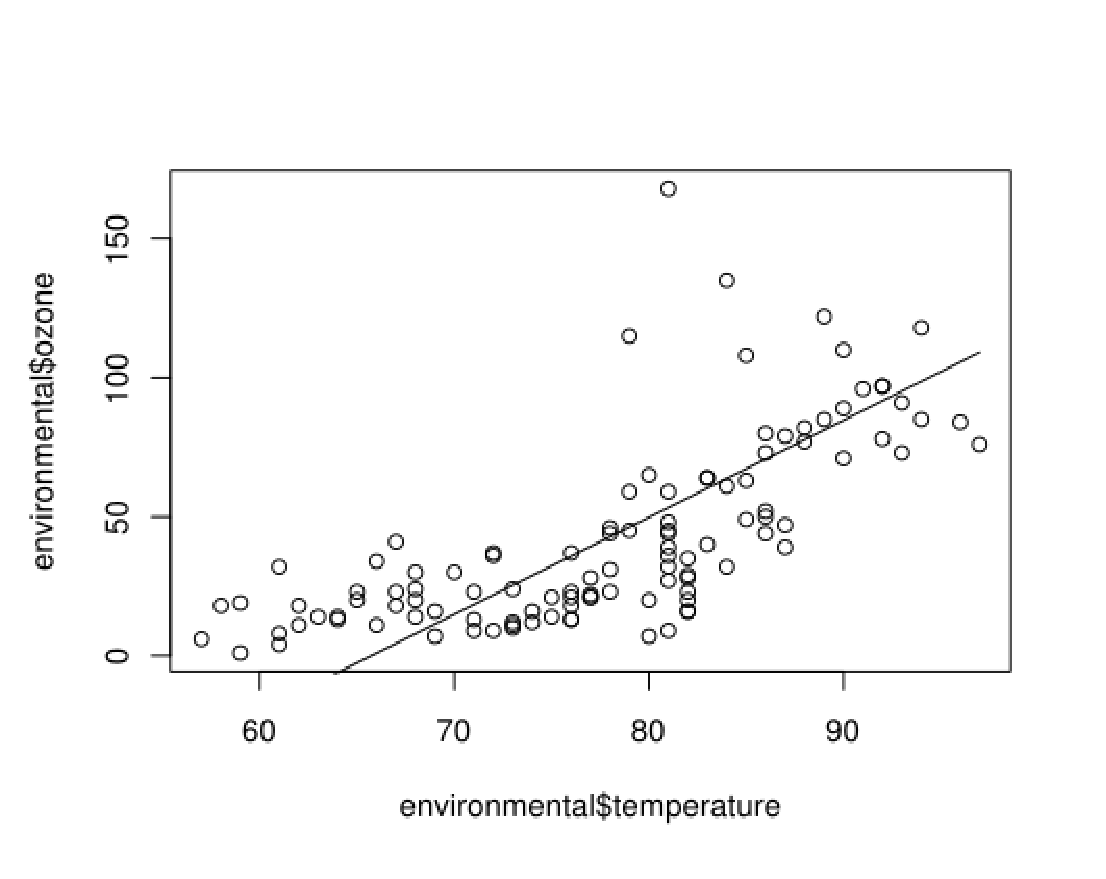
\includegraphics[height=4.2cm,bb=-0 -0 515 350,clip]{ozoneLine.eps}}
\psframe[linewidth=0.02,linecolor=gray](-6.2,-7)(6.2,2.2)
\psframe[linewidth=0.02,linecolor=gray](-6.15,-6.95)(6.15,2.15)
\rput(0,1.4){\color{myblue}\large Math 207:  Statistics}
\rput(0,0.6){\color{myblue}Chapter 8:  Correlation}
%\psframebox(0,0)(4,4)
\rput(0,-4.4){\scriptsize Dr.~Ralph Wojtowicz}
%\rput(0,-4.9){\scriptsize CME Department}
\rput(0,-5.6){
\includegraphics[height=2cm]{sulogolong.eps}}
%
%\rput(0,-6.5){\scriptsize 1 February 2012}
\end{pspicture}
\end{center}

\end{frame}

%\section[Outline]{}

\addtocounter{page}{-1}
\addtocounter{framenumber}{-1}

{\footnotesize
\frame{\tableofcontents}
}

\section{Scatter Diagrams}
\subsection{Scatter Diagrams}
\begin{frame}[t]\frametitle{Scatter Diagrams}
{\small
\begin{itemize}
\item Example from page 132 of our text\\
      \texttt{> x <- c(1, 3, 4, 5, 7)}\\
      \texttt{> y <- c(5, 9, 7, 1, 13)}\\
      \texttt{> plot(x, y)}
\rput(6,0){}
\item Example using an \texttt{R} environmental data set\\
      \texttt{> library(lattice)}\\
      \texttt{> plot(environmental\$temperature, environmental\$ozone)}\\
\end{itemize}%\vspace{-20pt}
}

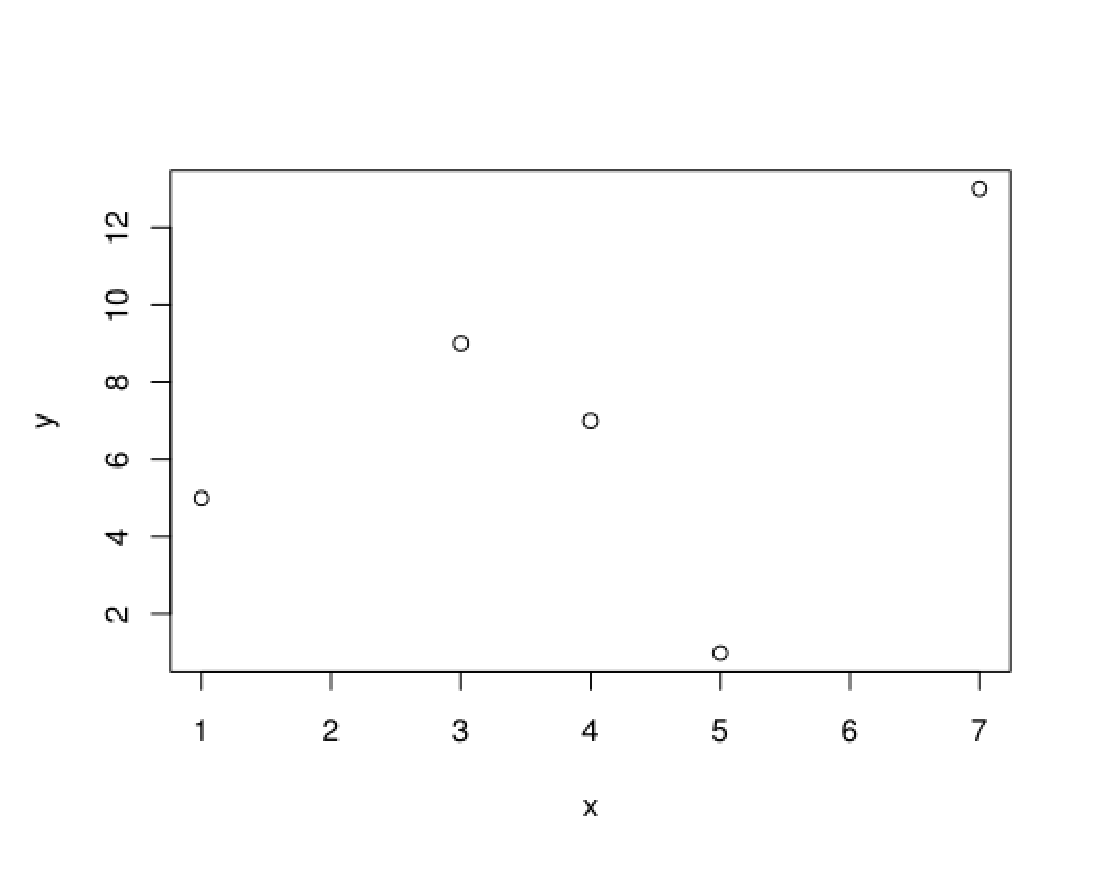
\includegraphics[height=4cm,bb=-0 -0 515 350,clip]{simpleData.eps}\hspace{0in}
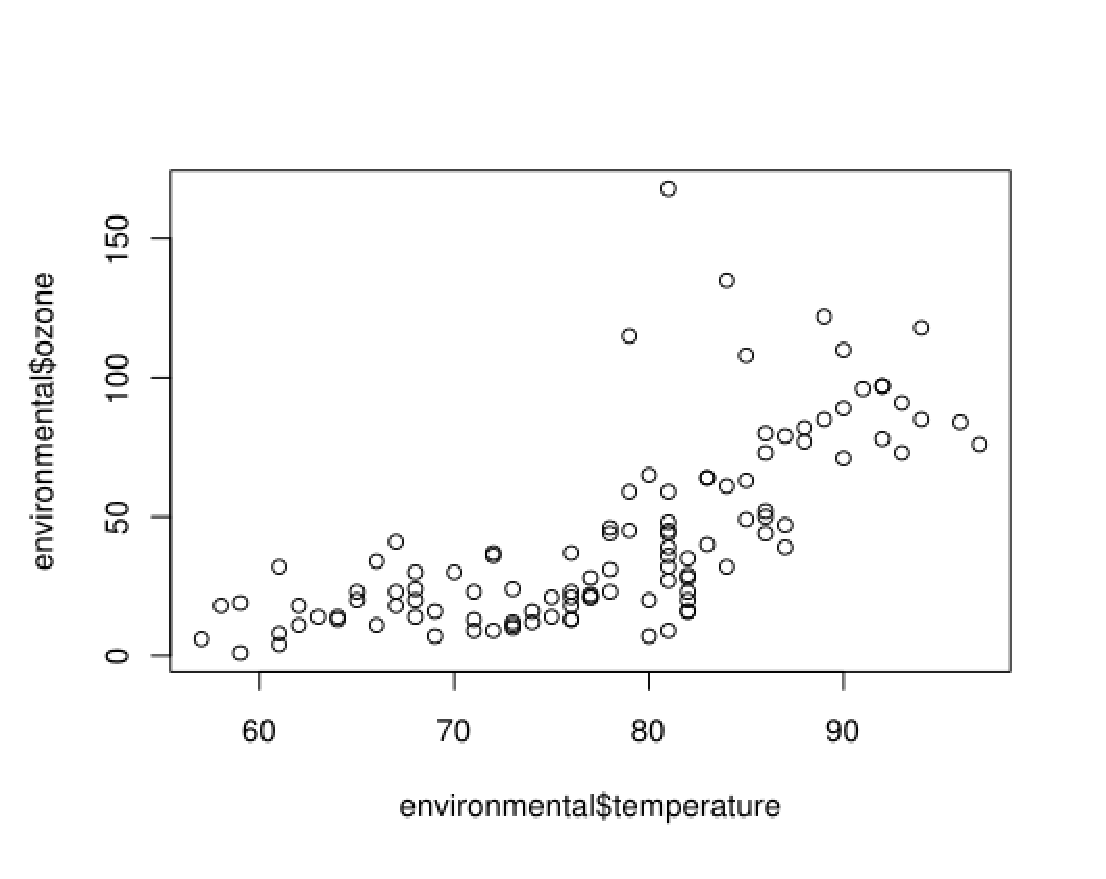
\includegraphics[height=4cm,bb=-0 -0 515 350,clip]{ozone.eps}
\end{frame}

\section{Correlation Coefficient}
\subsection{Correlation Coefficient}
\begin{frame}[t]\frametitle{The Correlation Coefficient}
{\small
\begin{itemize}
\item Given lists $x_1$, $\dots$, $x_n$ and $y_1$, $\dots$, $y_n$, the correlation
  coefficient:
  \begin{itemize} 
     \item Is a measure of linear association between the lists
     \item Is a measure of the clustering of the $(x_i, y_i)$ points around a line
     \item Is a number between $-1$ and $1$
     \item Is defined by:\vspace{-10pt}
   \end{itemize}
\end{itemize}
\begin{align*}
r &=\frac{1}{n}\,\sum_{i=1}^n\,\left(\frac{x_i - \mbox{mean}_x}{\mbox{SD}_x}\right)\,
  \left(\frac{y_i - \mbox{mean}_y}{\mbox{SD}_y}\right)\\
  &= \mbox{average of the $x$ and $y$ values measured in standard units}\vspace{-20pt}
\end{align*}\vspace{-15pt}
\begin{itemize}
\item A positive correlation means that the cloud of $(x_i, y_i)$ points slopes up
\item A negative correlation means that the cloud of $(x_i, y_i)$ points slopes down
\end{itemize}

}
\end{frame}

\subsection{Magnitude}
\begin{frame}
\frametitle{Magnitude of the Correlation Coefficient}

\begin{center}
\begin{pspicture}(0,0)(10,7)
%\psframe(0,0)(10,6)
\psline[linewidth=0.1,linecolor=purple]{<->}(0,6.5)(10,6.5)
\psline(5,6.7)(5,6.3)\rput(5,6.9){0.0}
\psline(0,6.7)(0,6.3)\rput(0,6.9){-1.0}
\psline(10,6.7)(10,6.3)\rput(10,6.9){1.0}
%
\rput(9,3){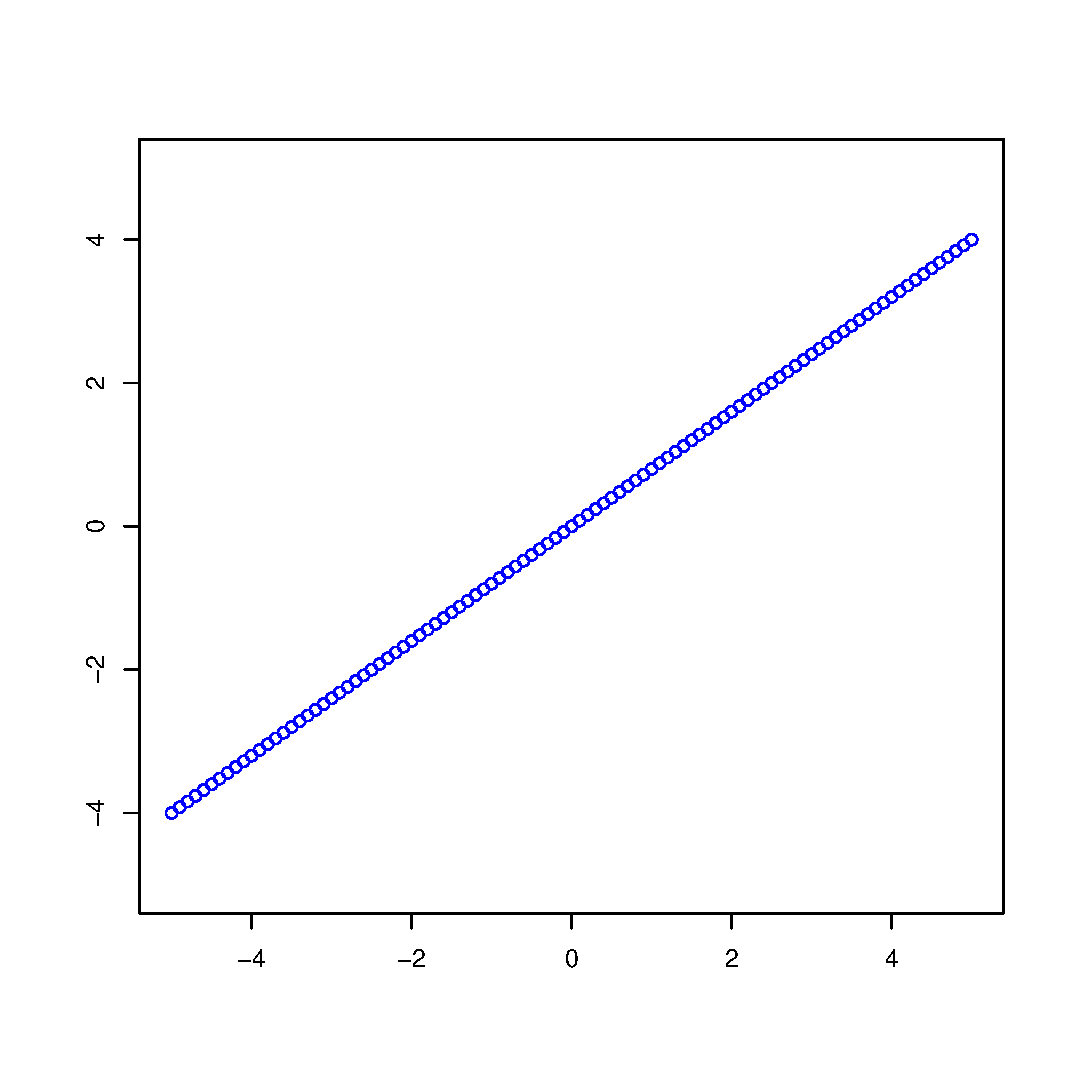
\includegraphics[height=1in]{cor1.eps}}    \rput(9,3.6){\footnotesize $r=1$}
\rput(7,1){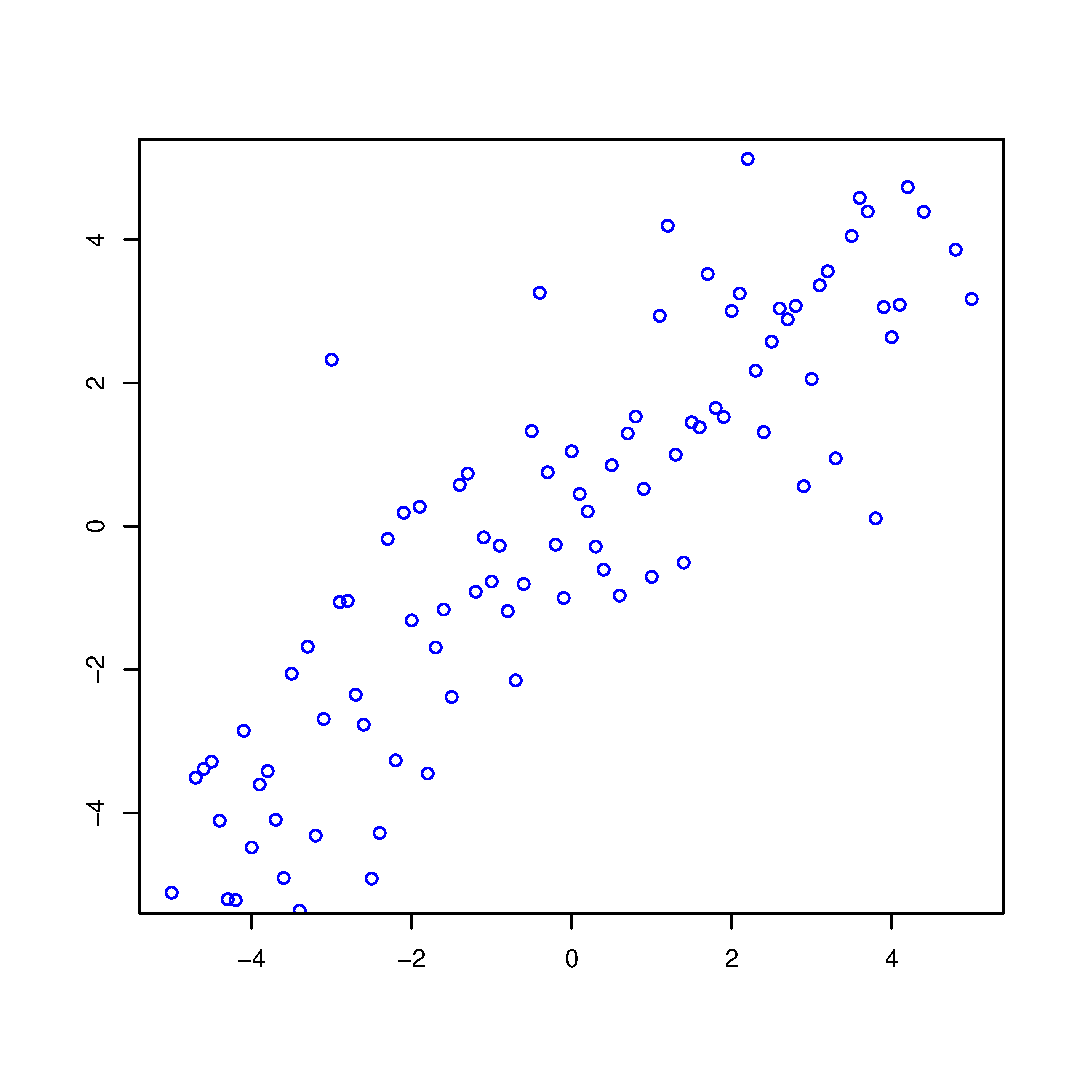
\includegraphics[height=1in]{cor_p9.eps}}  \rput(7,2.3){\footnotesize $r=0.9$}
\rput(6,5){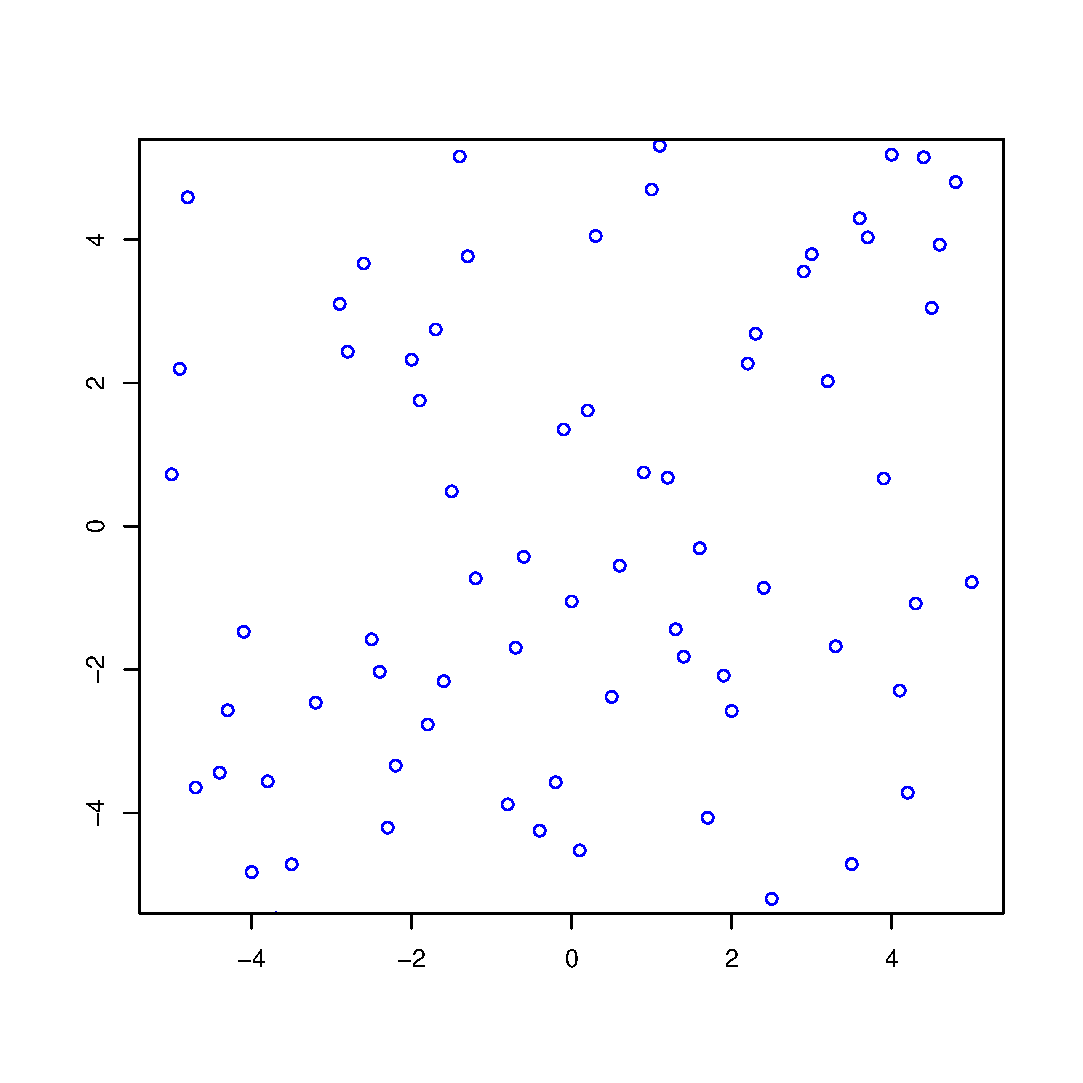
\includegraphics[height=1in]{cor_p4.eps}}  \rput(6,3.7){\footnotesize $r=0.4$}
%
\rput(4,1){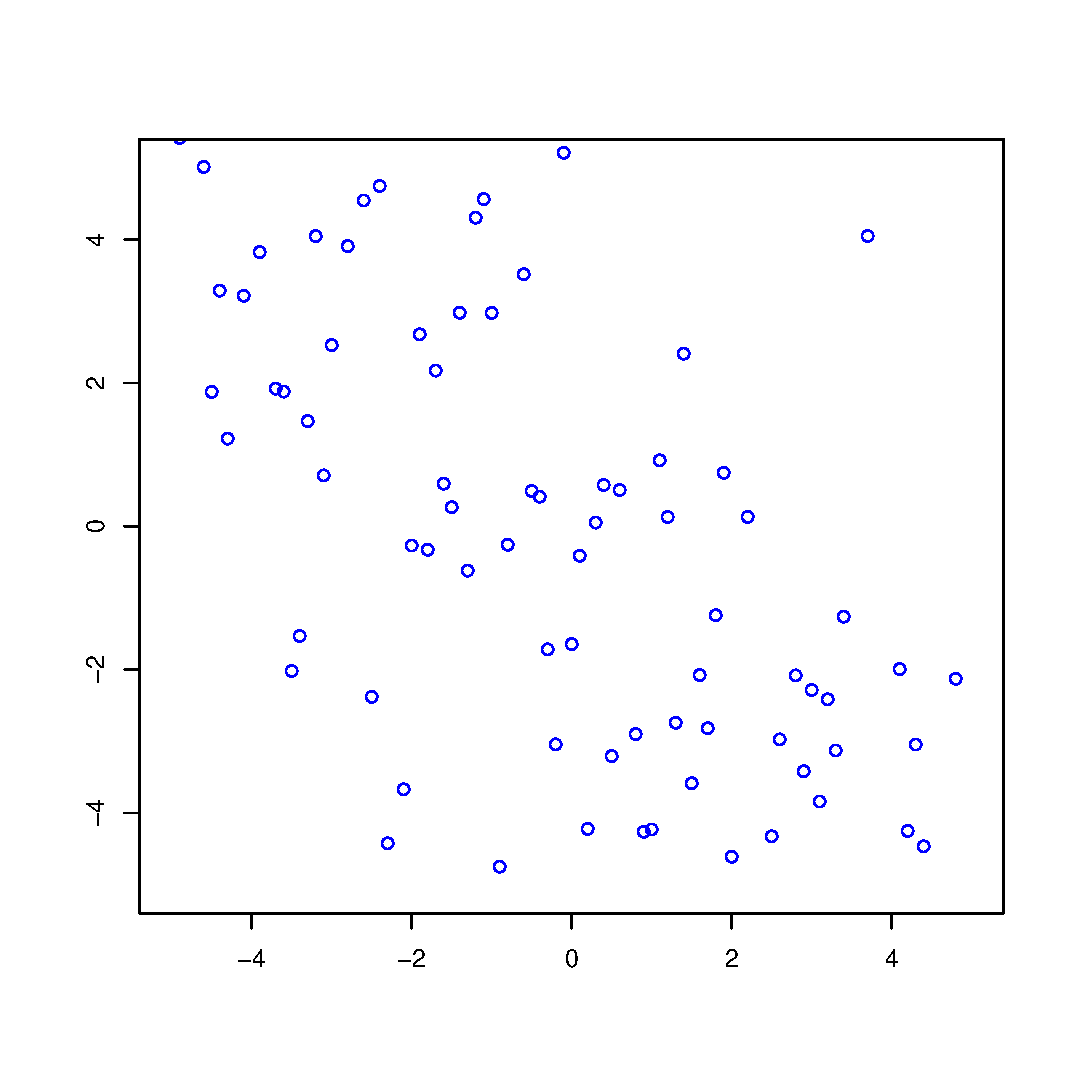
\includegraphics[height=1in]{cor_neg_p7.eps}} \rput(4,2.3){\footnotesize $r=-0.7$}
\rput(3,5){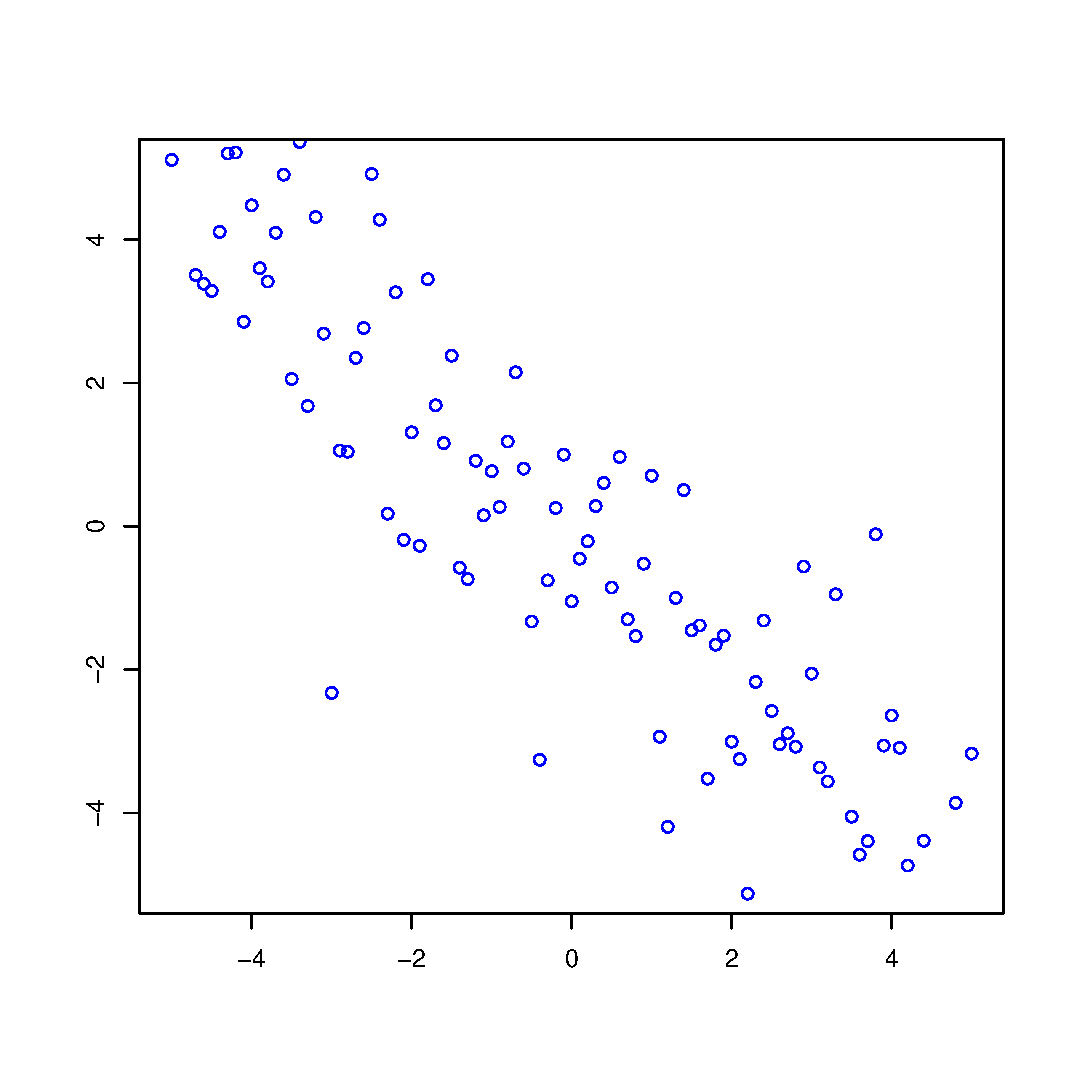
\includegraphics[height=1in]{cor_neg_p9.eps}} \rput(3.2,3.7){\footnotesize $r=-0.9$}
\rput(1,3){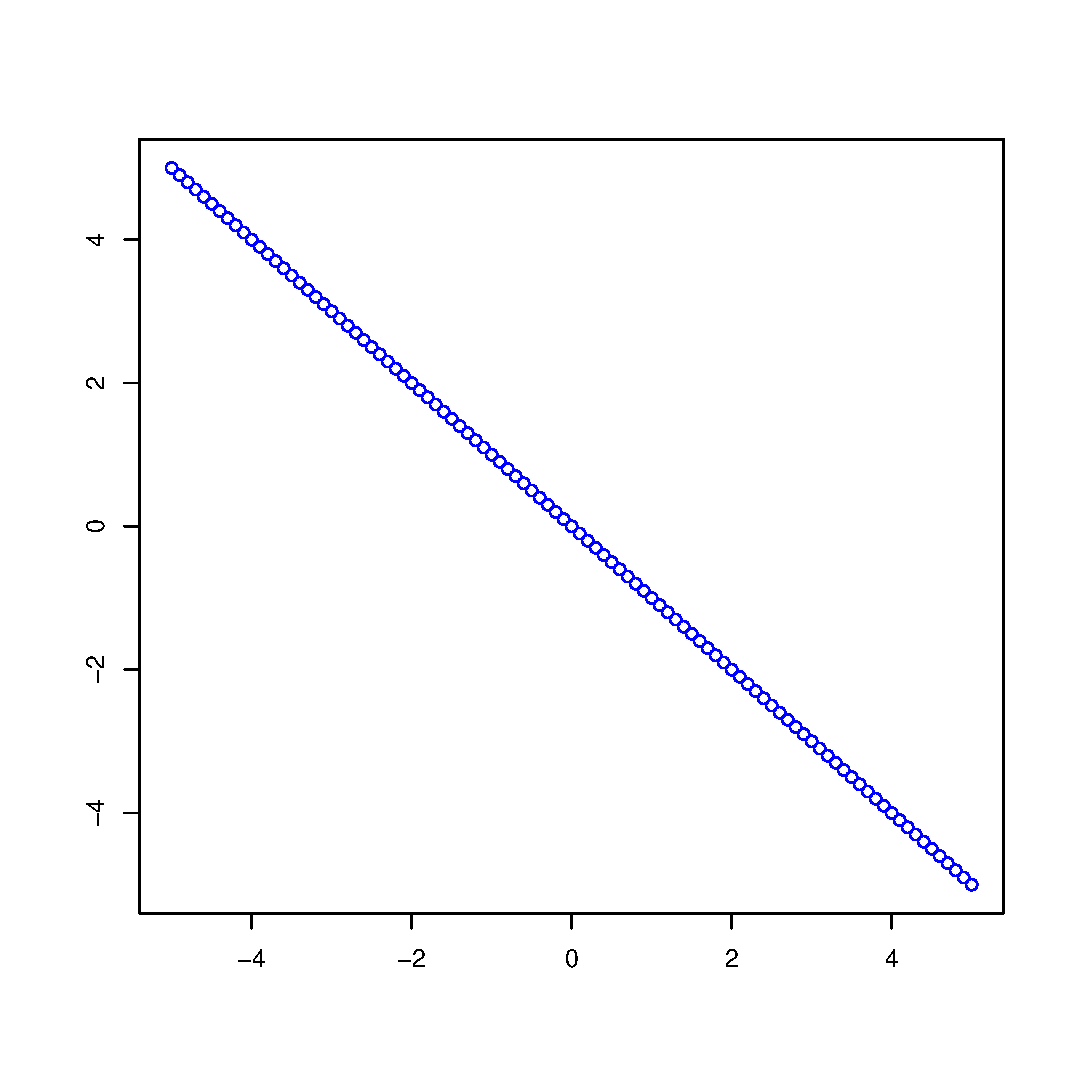
\includegraphics[height=1in]{cor_neg1.eps}} \rput(1,3.6){\footnotesize $r=-1$}
\end{pspicture}
\end{center}

\end{frame}

\subsection{Calculation}
\begin{frame}
\frametitle{Computing $r$}
\newcommand{\Z}{\hphantom{0}}
\newcommand{\VP}{\vphantom{\Large Y}}
\newcommand{\M}{\hphantom{$-$}}
\scriptsize
{\ }\vspace{-17pt}

\begin{center}
$\displaystyle r=\frac{1}{n}\sum \left(\frac{x_i - \mbox{mean}_x}{\mbox{SD}_x}\right)\!
   \left(\frac{y_i - \mbox{mean}_y}{\mbox{SD}_y}\right)$\hspace{10pt}
\begin{tabular}{|rr|ccc|}\hline
$x$ & $y$ & $z_x$ & $z_y$ & $z_x\,z_y$ \\[2pt]\hline
$1$   & $5$   & $-3/2$\M  & $-1/2$\M & $3/4$ \VP\\
$3$   & $9$   & $-1/2$\M  & $1/2$   & $-1/4$\M \\
$4$   & $7$   & $0$     & $0$     & $0$        \\
$5$   & $1$   & $1/2$   & $-3/2$\M  & $-3/4$\M  \\
$7$   & $13$  & $3/2$   & $3/2$   & $9/4$       \\\hline
\end{tabular}\vspace{-8pt}
\end{center}
\tiny
\uncover<2->{\begin{align*}
\mbox{mean}(x) & = \frac{1}{5}\,(1 + 3 + 4 + 5 + 7) = 4 \hspace{14pt}
\mbox{SD}(x)    = \sqrt{\frac{(1-4)^2 + (3-4)^2 + (4-4)^2 + (5-4)^2 + (7-4)^2}{5}} 
   %\sqrt{\frac{9 + 1 + 0 + 1 + 9}{5}} = 
    %\sqrt{\frac{20}{5}}=\sqrt{4} 
                =2\\[-1pt]
\mbox{mean}(y) &=\frac{1}{5}\,(5 + 9 + 7 + 1 + 13) = 7 \hspace{10pt}
\mbox{SD}(y)   =\sqrt{\frac{(5-7)^2 + (9-7)^2 + (7-7)^2 + (1-7)^2 + (13-7)^2}{5}}
     %= \sqrt{\frac{4 + 4 + 0 + 36 + 36}{5}} 
   %= \sqrt{\frac{80}{5}}  
  = 4
\end{align*}}\vspace{-2pt}
\begin{itemize}
\item<3-> Convert the $x$ values to standard units.  For example,\vspace{-3pt}
\[x = 1\mbox{\hspace{10pt}becomes\hspace{10pt}} z_x = \frac{1-4}{2} = -3/2
\mbox{\hspace{20pt}and\hspace{20pt}}
x = 3\mbox{\hspace{10pt}becomes\hspace{10pt}} z_x = \frac{3-4}{2} = -1/2\]
\item<4-> Convert the $y$ values to standard units:
For example,\vspace{-3pt}
\[y=5\mbox{\hspace{10pt}becomes\hspace{10pt}} z_y=\frac{5-7}{4} = -1/2
\mbox{\hspace{20pt}and\hspace{20pt}}
y=9\mbox{\hspace{10pt}becomes\hspace{10pt}}  z_y = \frac{9-7}{4} = 1/2\vspace{-5pt}\]
\item<5-> Compute the products $z_x\,z_y$.
\item<6-> Compute the correlation coefficient:
{\color{blue}$r = \frac{1}{5}\,\left(\frac{3}{4} - \frac{1}{4} + 0 - \frac{3}{4} + \frac{9}{4}\right)
  = \frac{1}{5}\,\frac{8}{4} = \frac{2}{5} = 0.4$}
\item<7-> In R:\begin{tabular}{l}
\texttt{x <- c(1, 3, 4, 5, 7)}\\
\texttt{y <- c(5, 9, 7, 1, 13)}\\
\texttt{cor(x, y)}
\end{tabular}
\end{itemize}

\end{frame}

\section{The SD Line}
\subsection{The SD Line}
\begin{frame}[t]\frametitle{The SD Line}
{\small
\begin{itemize}
\item Given lists $x_1$, $\dots$, $x_n$ and $y_1$, $\dots$, $y_n$, the SD line  
   \begin{itemize}
   \item Is a linear approximation to the cloud of $(x_i, y_i)$ points
   \item Is defined by\vspace{-10pt}
\[\left(y - \mbox{mean}_y\right) = \left(\mbox{sign $r$}\right)\,
   \left(\frac{\mbox{SD}_y}{\mbox{SD}_x}\right)\,\left(x - \mbox{mean}_x\right)\vspace{-3pt}\]
 where $r$ is the  correlation coefficient.\vspace{2pt}
   \item It goes through the point of averages:  $(\mbox{mean}_x,\; \mbox{mean}_y)$.
   \item It's slope is $\pm\;\frac{\mbox{\scriptsize SD}_y}{\mbox{\scriptsize SD}_x}$.
   \end{itemize}
\item For every increase of 1 $\mbox{SD}_x$ in the $x$-direction, there is an increase of 1 
$\mbox{SD}_y$   in the $y$-direction.
\item If  $r>0$, the slope of the SD line is $\hphantom{-}
\frac{\mbox{\scriptsize SD}_y}{\mbox{\scriptsize SD}_x}$.
\item If  $r<0$, the slope of the SD line is $-\frac{\mbox{\scriptsize SD}_y}{\mbox{\scriptsize SD}_x}$.
\end{itemize}
}
\end{frame}

\subsection{Calculation}
\begin{frame}
\frametitle{SD Line Calculation}
\newcommand{\Z}{\hphantom{0}}
\newcommand{\VP}{\vphantom{\Large Y}}
\newcommand{\M}{\hphantom{$-$}}
{\ }\vspace{-28pt}

{\scriptsize
\begin{center}
\begin{tabular}{|rr|ccc||cc|}\hline
    &     &       &       &           & $y$ values   & \VP\\
    &     &       &       &           &  predicted  & SD\\
$x$ & $y$ & $z_x$ & $z_y$ & $z_x\,z_y$ & by SD line  & error\\[2pt]\hline
$1$   & $5$   & $-3/2$\M  & $-1/2$\M  & $3/4$       &  1  & 4\VP\\
$3$   & $9$   & $-1/2$\M  & $1/2$   & $-1/4$\M      &  5  & 4\\
$4$   & $7$   & $0$     & $0$     & $0$         &  7  & 0\\
$5$   & $1$   & $1/2$   & $-3/2$\M  & $-3/4$\M      &  9  & $-8$\M\\
$7$   & $13$  & $3/2$   & $3/2$   & $9/4$       &  13 & 0\\ \hline
\end{tabular}\vspace{-10pt}
\end{center}

\begin{itemize}
\item SD line equation:\\
$\displaystyle \left(y - \mbox{mean}_y\right) = \left(\mbox{sign $r$}\right)\,
   \left(\frac{\mbox{SD}_y}{\mbox{SD}_x}\right)\,\left(x - \mbox{mean}_x\right)$
\item Subsitute the values from Slide 5:\\[3pt]
$\displaystyle\left(y - 7\right) = (+1)\,
   \left(\frac{4}{2}\right)\,\left(x - 4\right)$\\[5pt]
which simplifies to\\[2pt]
{\color{blue}$(y-7) = 2\,(x-4)$}
\end{itemize}
}

\rput(9.2,1.7){\begin{pspicture}(0,0)(4,4)
\psset{xunit=0.57143, yunit=0.30769}
\psline[linewidth=0.02](0,0)(7,0)
\rput(1,-0.7){\scriptsize 1}
\rput(2,-0.7){\scriptsize 2}
\rput(3,-0.7){\scriptsize 3}
\rput(4,-0.7){\scriptsize 4}
\rput(5,-0.7){\scriptsize 5}
\rput(6,-0.7){\scriptsize 6}
\rput(7,-0.7){\scriptsize 7}
%
\psline[linewidth=0.02](0,0)(0,13)
\rput[r](-0.2,1){\scriptsize 1}
\rput[r](-0.2,2){\scriptsize 2}
\rput[r](-0.2,3){\scriptsize 3}
\rput[r](-0.2,4){\scriptsize 4}
\rput[r](-0.2,5){\scriptsize 5}
\rput[r](-0.2,6){\scriptsize 6}
\rput[r](-0.2,7){\scriptsize 7}
\rput[r](-0.2,8){\scriptsize 8}
\rput[r](-0.2,9){\scriptsize 9}
\rput[r](-0.2,10){\scriptsize 10}
\rput[r](-0.2,11){\scriptsize 11}
\rput[r](-0.2,12){\scriptsize 12}
\rput[r](-0.2,13){\scriptsize 13}
%
\psline[linecolor=blue,linewidth=0.02](1,1)(7,13)\rput[br](6.1,11.5){\scriptsize SD line}
\psline[linecolor=darkgreen,linewidth=0.02,linestyle=dashed](1,4.6)(7,9.4)
    \rput[lt](5.5,7.9){\scriptsize Regression line}
\psdot(1,5)
\psdot(3,9)
\psdot*[linecolor=red](4,7)
\psdot(5,1)
\psdot(7,13)
\end{pspicture}}

\label{lastpage}
\end{frame}

\end{document}

\vspace{-4pt}
   \end{itemize}
\end{itemize}
\[\left(y - \mbox{mean}_y\right) = \left(\mbox{sign $r$}\right)\,
   \left(\frac{\mbox{SD}_y}{\mbox{SD}_x}\right)\,\left(x - \mbox{mean}_x\right)\]\vspace{-10pt}
\begin{itemize}
\item Here is an example in \texttt{R} (see page 132 of our text)\\
\texttt{> x <- c(1, 3, 4, 5, 7)}\\
\texttt{> y <- c(5, 9, 7, 1, 13)}\\
\texttt{> source("http://www.adjoint-functors.net/SDline.R")}\\
\texttt{> SDline(x, y)}\\
\texttt{> \$meanX}\hspace{30pt}\texttt{> \$meanY}\\
\texttt{>[1] 4}\hspace{37pt}   \texttt{>[1] 7}\\
\texttt{> \$slope}\hspace{30pt}\texttt{> \$correlation}\\
\texttt{>[1] 2}\hspace{37pt}   \texttt{>[1] 0.4}\\
